\documentclass{simcenterdocumentation}
\usepackage[sorting=none, backend=biber]{biblatex}
\usepackage{subfig}
\usepackage{multirow}
\usepackage{adjustbox} % to adjust table width
\usepackage{graphicx} %Loading the package
\usepackage{longtable}
\usepackage{cleveref}
\graphicspath{{../Common/}{.}} %Setting the graphicspath
\makeatletter % Search additional directories for inputs
\def\input@path{{../Common/}{.}}
%or: \def\input@path{{/path/to/folder/}{/path/to/other/folder/}}
\makeatother

%% Add unicode support for special characters
%%\usepackage[utf8x]{inputenc}

% To compile this file, run "latex/pdflatex codedoc", then "biber codedoc"b
% (or "bibtex codedoc", if the output from latex asks for that instead),
% and then "latex/pdflatex codedoc" (without the quotes in each case).

% Double spacing, if you want it.  Do not use for the final copy. Can also specify
% draft as a document class option. This will generate double spacing and placeholders
% for title page and header images
%% \def\dsp{\def\baselinestretch{2.0}\large\normalsize}
%% \dsp

\bibliography{../Common/references}

\begin{document}
% Declarations for Front Matter
% Software title followed by optional second line
\title{PBE\\ Performance-Based Engineering Application}
% Use superscripts to indicate author affiliations
\author{Frank McKenna, Adam Zsarn\'oczay, \\ Wael Elhaddad, Chaofeng Wang, and Michael Gardner}
\institutions{NHERI SimCenter, UC Berkeley}
\softwarename{PBE}
\softwareversion{1.2}
\softwarepage{https://simcenter.designsafe-ci.org/research-tools/pbe-application/}

%%% DON'T MESS WITH THESE SETTINGS %%%%%%%%%%%%%%%%%%%%%%%%%%%%%%%%
\hypersetup{pageanchor=false}
\maketitle
\copyrightpage
\acknowledgments

\hypersetup{pageanchor=true}
\begin{frontmatter}

\pagestyle{plain}
{
  \renewcommand{\thispagestyle}[1]{}
  \tableofcontents
  \clearpage
  \listoffigures
  \clearpage
  \listoftables
}

\end{frontmatter}
\pagestyle{somewhatsimple}
%%%%%%%%%%%%%%%%%%%%%%%%%%%%%%%%%%%%%%%%%%%%%%%%%%%%%%%%%%%%%%%%%%%
% Create separate tex files for each chapter and provide them as inputs

\chapter{About}
\label{chap:about}
The intended audience for the \texttt{\getsoftwarename{}} Application (\texttt{\getsoftwarename{}} App) is researchers and practitioners
interested in quantification of the seismic performance of buildings.\\

This is an open-source, research application. The source code at
the \href{https://github.com/NHERI-SimCenter/PBE}{\texttt{\getsoftwarename{}}
Github page} provides an application that can be used to assess the performance of a building in an earthquake scenario. The application focuses on quantifying building performance through decision variables. Given that the properties of the buildings and the earthquake events are not known exactly, and that the simulation software and the user make simplifying assumptions in when modeling the seismic event and the structural response, the estimated response of the structure already exhibits significant variability. Structural response and its uncertainty can be estimated using our \href{https://simcenter.designsafe-ci.org/research-tools/ee-uq-application/}{\texttt{EE-UQ} Application}. The \texttt{\getsoftwarename{}} App builds on the \texttt{EE-UQ} App and uses its response estimates to assess the damage to building components and the consequences of such damage.\\

The user can characterize the structural model, the damage and loss model, and the seismic hazard model in this application. All models are interconnected by an uncertainty quantification framework that allows the user to define a stochastic model for the problem. Given that stochastic model, the application first performs nonlinear response-history simulations to obtain the Engineering Demand Parameters (EDPs) that describe structural response. Then, those EDPs are used to assess the Damage Measures (DMs) and Decision Variables (DVs) that characterize building performance.\\

Depending on the type of structural system, the fidelity of the structural model, and the number of EDP samples, the response-history simulations can be computationally prohibitively expensive. To overcome this impediment, the user can choose to perform the response simulations on the Stampede2 supercomputer. Stampede2 is located at the Texas Advanced Computing Center (TACC) and made available to the user through NHERI DesignSafe-CI, the cyberinfrastructure provider for the distributed, NSF-funded, Natural Hazards Engineering Research Infrastructure (NHERI) facility.\\

The computations are performed, as will be discussed in \Cref{chap:theory}, with a Workflow Application. A Workflow Application is a sequence of tools linked together. The \texttt{\getsoftwarename{}} backend runs those tools, taking the outputs from some programs and providing them as inputs to others. Researchers can extend the Workflow Application to use their own tools in the backend computations. This ensures that researchers are not limited to using the default applications we provide and will be enthused to provide their own applications for others to use.\\

This is Version \getsoftwareversion{} of the tool. Users are
encouraged to comment on what additional features and capabilities
they would like to see in this application. These requests and
feedback can be submitted through an anonymous \insertsurveylink{user
survey}; we greatly appreciate any input you have. If there are
features you want, chances are many of your colleagues also would
benefit from them. Users are encouraged to review
\Cref{chap:requirements} to see what features are planned for future releases.


\chapter{Installation Instructions}
\label{chap:installation}
All SimCenter applications are available at
the \href{https://simcenter.designsafe-ci.org/research-tools/overview/}{SimCenter
website} under \emph{Research Tools}. The following sections outline
the steps necessary to download and install the \texttt{\getsoftwarename{}}
application. The SimCenter applications do require that you install a
number of other applications that are needed to run the workflows on
your local machine as well as at DesignSafe. \\


%===============================================================================
\section{Download the Application}
%===============================================================================

% \subsection{Download the Application Files}

To download the \texttt{\getsoftwarename{}} application navigate to
the \getsoftwarepage{\texttt{\getsoftwarename{}} page} and click on
the \emph{Download App \& User Manual} link on the right side of the
page. As shown in \Cref{fig:app_choose_file}, this will take you to another page which contains a list of downloadable files and directories.

\softwareSwitch{PBE}{
\begin{figure}[!htbp]
  \centering {
    \includegraphics[width=0.95\textwidth]
    {Common/installation/figures/pbeDownload.png} }
  \caption{Download Application}
  \label{fig:app_choose_file}
\end{figure}
}{}

\softwareSwitch{EE-UQ}{
\begin{figure}[!htbp]
  \centering {
    \includegraphics[width=0.95\textwidth]
    {installation/figures/eeDownload.png} }
  \caption{Download Application}
  \label{fig:app_choose_file}
\end{figure}
}{}

\softwareSwitch{WE-UQ}{
\begin{figure}[!htbp]
  \centering {
    \includegraphics[width=0.95\textwidth]
    {installation/figures/eeDownload.png} }
  \caption{Download Application}
  \label{fig:app_choose_file}
\end{figure}
}{}


There are at least four files available for download from this page: 
\begin{enumerate}
    \item The PDF file is the User Manual that you are reading now.
    \item The MOV file is a video that provides an introduction to the usage of the application.
    \item The ZIP file is an archive that contains the application files for a Windows operating system.
    \item The DMG file is an archive that contains the application files for a Mac OS X operating system.
\end{enumerate}

To download the \texttt{\getsoftwarename{}} application click on the link for
the appropriate file for your operating system and then click on the
Download button at bottom right corner of the pop-up window. 
Unpackage the application from the downloaded
file and place it in a location on your filesystem. On Windows, we
recommend that you create a \texttt{C:/SimCenter/\getsoftwarename{}}
directory and extract the contents of the \texttt{ZIP} archive
there. It is also recommended to run the included installer for Visual C/C++ runtime library(vc\_redist.x64.exe). 
If you use a Mac we recommend you copy the application to either your
Documents folder or your Desktop folder. You are free to place the
applications anywhere you wish, you will need to make the
appropriate adjustments with the following instructions if you do so. \\

Now test if the application starts. To do this navigate to
the location where you placed the application and open it. You should
see the user interface (UI) shown in \Cref{fig:app_UI} after
starting the application. Now Quit the application. Additional steps are required before 
computations can be performed.\\

\softwareSwitch{PBE}{
\begin{figure}[!htbp]
  \centering {
    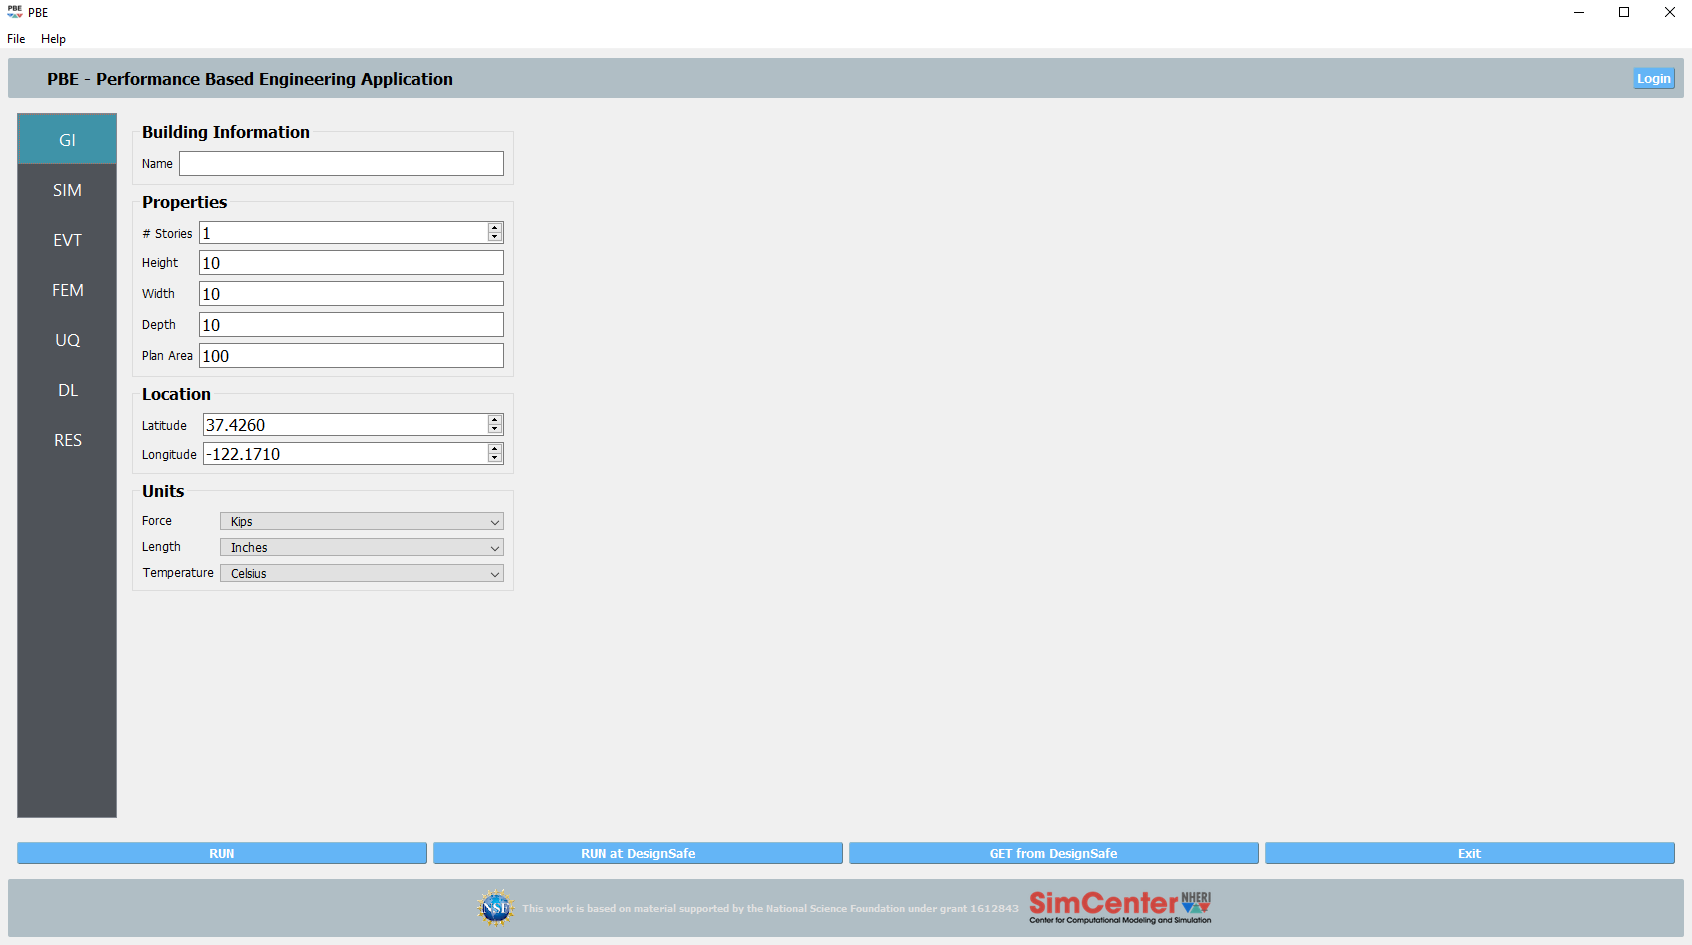
\includegraphics[width=1.00\textwidth]
    {installation/figures/PBE.png} }
  \caption{PBE Application on Startup}
  \label{fig:app_UI}
\end{figure}
}{}

\softwareSwitch{EE-UQ}{
\begin{figure}[!htbp]
  \centering {
    \includegraphics[width=0.95\textwidth]
    {installation/figures/EE-UQ.png} }
  \caption{EE-UQ Application on Startup}
  \label{fig:app_UI}
\end{figure}
}{}

\softwareSwitch{WE-UQ}{
\begin{figure}[!htbp]
  \centering {
    \includegraphics[width=0.95\textwidth]
    {installation/figures/EE-UQ.png} }
  \caption{WE-UQ Application on Startup}
  \label{fig:app_UI}
\end{figure}
}{}


\begin{enumerate}
\item The SimCenter is not recognized as either a Windows or an Apple vendor. Our applications are not recognized by the operating system as being signed. Consequently, you may receive a warning message when you start the \texttt{\getsoftwarename{}} application for the first time.
\item  On a Mac you will need to right click on the .dmg file to open it. The UI will not start correctly while in the DMG file, you need to open the .dmg file and then copy the \texttt{\getsoftwarename{}} application to your Documents or Desktop folder. You can then move the .dmg file to the trash or eject it after this has been done.
\item  The \texttt{\getsoftwarename{}} application requires additional software outlined in next sections to work properly. Even though it starts correctly, it will not run the simulations until other software, outlined in the next section, is installed.
\end{enumerate}


%===============================================================================
\section{Set up Python}
%===============================================================================

The SimCenter workflow applications are managed by Python
scripts. These are required to prepare the input data for running
analyses either remotely on DesignSafe or locally. Consequently, the user must have Python
installed on their machine and have the appropriate environment
variables set so that the UI can run these applications.

\subsection{Install Python}

If you have not yet installed Python, we recommend
installing \href{http://www.anaconda.com/distribution/#download-section}{Anaconda}. Anaconda
provides all the important scientific packages in a single convenient
install. We recommend installing the 64-Bit version based on Python
3.5 or newer.

Note: If you already have a Python installation that is Python 2.7 or
newer, you do not have to install Anaconda to work with SimCenter
applications.
If you take this approach, please make sure that you also have the following packages installed: 
\texttt{numpy}, \texttt{scipy}, and \texttt{pandas}.

\subsection{Test Python}
%===============================================================================

Test if the Python environment is set up properly by
executing \texttt{python} in a terminal window. After Python starts,
test if the packages are installed by executing \texttt{import
numpy}, \texttt{import scipy}, and \texttt{import pandas}. You will
receive an error message if a pacakage is missing. If no error
appears, the terminal should look similar
to \Cref{fig:python_test}. Exit Python by executing
the \texttt{exit()} command.

\begin{figure}[!htbp]
  \centering {
    \includegraphics[width=0.8\textwidth]
    {installation/figures/python_test.png} }
  \caption{Testing the Python environment.}
  \label{fig:python_test}
\end{figure}

%===============================================================================
\section{Set up for Running Workflows Locally}\label{setup}
%===============================================================================

To run the workflows locally, the backend python application needs
publicly available software to also be installed on your
machine. These software applications need to be installed and
configured on your operating system. If you do not plan to run the
workflows locally, you will not need these applications.

\subsection{Install \texttt{OpenSees}}
%===============================================================================

\href{http://opensees.berkeley.edu}{\texttt{OpenSees}} is an open-source finite element application publicly available for download from its \href{http://opensees.berkeley.edu/OpenSees/user/download.php}{download page}. \texttt{OpenSees} installation requires the user install both \texttt{OpenSees} and \texttt{Tcl}.  If you have never downloaded \texttt{OpenSees} before, you will need to register your e-mail to gain access. After registration, you can proceed to the download page by entering your email address and clicking the Submit button. The Windows and Mac downloads are in different locations on the download page, with the appropriate Tcl installer beside the \texttt{OpenSees} link; see \Cref{fig:openseesDownload}

\begin{figure}[!htbp]
  \centering {
    \includegraphics[width=\textwidth]
    {installation/figures/openseesDownload.png} }
  \caption{Downloading OpenSees}
  \label{fig:openseesDownload}
\end{figure}

Follow the instructions on the download page to install \texttt{Tcl}
(\Cref{fig:openseesDownload}). On Windows, you must select the Custom option for installton and you must specify
the installtion directory as \texttt{C:\textbackslash Program Files\textbackslash Tcl}, 
which is not the default. \\

After \texttt{Tcl} is installed, we recommend you put \texttt{OpenSees} in
the \texttt{C:/SimCenter/OpenSees} folder on Windows and in
a \texttt{/usr/local/OpenSees} directory on the Mac (If you use finder
on Mac to do navigation, use command-shift-G in Finder and specify
/usr/local as the folder to go to. Create a new folder \texttt{OpenSees}
and copy the \texttt{OpenSees} application to this folder).\\


Now you need to add the \texttt{OpenSees} folder to the
system \texttt{PATH} environment variable to allow the SimCenter
workflow applications to find the \texttt{OpenSees} executable on your
computer. The steps to do this depend on your operating system:

\begin{enumerate}
\item Windows: To add a folder to the \texttt{PATH} on Windows (\Cref{fig:add_env_path}):

\begin{figure}[!htbp]
  \centering {
    \includegraphics[width=0.8\textwidth]
    {installation/figures/add_env_path.png} }
  \caption{Adding OpenSees to the PATH environment variable on Windows}
  \label{fig:add_env_path}
\end{figure}


\begin{enumerate}
    \item open \emph{Start}, type \emph{env}, and choose \emph{Edit the system environment variables};
    \item click on the \emph{Environment variables...} button in the dialog window;
    \item find the \texttt{Path} under \emph{System Variables} in the \emph{Variable} column;
    \item click \emph{New} and type in the path to your \texttt{OpenSees.exe} (this will be \texttt{C:\textbackslash SimCenter\textbackslash OpenSees} if you put the executable at the recommended location - pay attention to using backslashes here!);
    \item click \emph{OK} in every dialog to close them and save your changes.
\end{enumerate}

\item MacOS: To add the /usr/local/OpenSees folder to the \texttt{PATH} variable:


\begin{enumerate}
    \item open a Terminal;
    \item execute \texttt{sudo nano /etc/paths} and enter your password
    \item add the path to the \texttt{OpenSees} executable to the end of the list (this will be \texttt{/usr/local/OpenSees} if you put the executable at the recommended location);
    \item quit by hitting \texttt{Ctrl+X} and then \texttt{Y} when asked if you want to save modifications.
\end{enumerate}

\begin{figure}[!htbp]
  \centering {
     \includegraphics[width=0.8\textwidth]
    {installation/figures/add_env_path_Mac.png} }
  \caption{Adding OpenSees to the PATH environment variable on Mac.}
  \label{fig:add_env_path_Mac}
\end{figure}
\end{enumerate}


\subsection{Install \texttt{Dakota}}
%===============================================================================

\href{http://dakota.sandia.gov}{\texttt{Dakota}}, an open-source  optimization and UQ application from Sandia National Labs, is publicly available for download at its \href{http://dakota.sandia.gov/download.html}{download page}. Select your operating system from the list and set the other options as shown in  \Cref{fig:dakota_installation}. Download the release in a \texttt{ZIP} file for Windows and \texttt{TAR.GZ} file for Mac. We recommend you to extract the archive to a \texttt{C:/SimCenter/Dakota} folder on Windows, and to a \texttt{/usr/local/Dakota} folder on a Mac.

\begin{figure}[!htbp]
  \centering {
    \includegraphics[width=\textwidth]
    {installation/figures/dakota_installation.png} }
  \caption{Downloading Dakota Software}
  \label{fig:dakota_installation}
\end{figure}

Following the instructions provided for installing \texttt{OpenSees}, you need to add \textbf{two} \texttt{Dakota} folders to the system \texttt{PATH} environment variable to allow the SimCenter
workflow applications to find the \texttt{Dakota} tools on your computer. Use
the procedure described above for \texttt{OpenSees} to add the following
folders to your \texttt{PATH}:

\begin{enumerate}
\item Windows:
\begin{itemize}
    \item \texttt{C:\textbackslash SimCenter\textbackslash Dakota\textbackslash bin}
    \item \texttt{C:\textbackslash SimCenter\textbackslash Dakota\textbackslash share\textbackslash dakota\textbackslash Python}
\end{itemize}

\item MacOS:
\begin{itemize}
    \item \texttt{/usr/local/Dakota/bin}
    \item \texttt{/usr/local/Dakota/share/dakota/Python}
\end{itemize}
\end{enumerate}

In addition to modifications to the \texttt{PATH} environment variable, you need to create/modify another variable. This new variable name is \texttt{PYTHONPATH}. To add an environment variable on a Mac you need to edit the \texttt{.bashrc} file in your home directory and add the line shown below.

\begin{enumerate}
\item Windows:
\begin{itemize}
    \item \texttt{C:\textbackslash SimCenter\textbackslash Dakota\textbackslash share\textbackslash dakota\textbackslash Python}
\end{itemize}

\item MacOS:
\begin{itemize}
    \item \texttt{export PYTHONPATH=/usr/local/Dakota/share/dakota/Python}
\end{itemize}
\end{enumerate}

\subsection{Install  Perl}
%===============================================================================

Mac OS X has Perl pre-installed, but Windows users will have to
install it to be able to use \texttt{Dakota}. We recommend you use Strawberry
Perl; you can install it by downloading the executable from
its \href{http://strawberryperl.com}{Strawberry Perl website} and
running it.

\subsection{Test the Install of the Local Applications}
%===============================================================================

Before running the \texttt{\getsoftwarename{}} application, perform the following tests to
make sure that the local SimCenter working environment is set up
appropriately:

\begin{itemize}
    \item Start a Terminal on Mac or a Command Prompt on Windows.
    \item On Mac, execute \texttt{cd /usr/Documents} to change the active directory to \texttt{/usr/Documents}. On Windows, execute \texttt{cd C:/} to change the active directory to \texttt{C:/}.
    \item Test if \texttt{OpenSees} works correctly by executing the \texttt{OpenSees} command. The command should start \texttt{OpenSees} (\Cref{fig:opensees_test}). Close \texttt{OpenSees} with the \texttt{exit} command.
    \item Test if \texttt{Dakota} works correctly by executing the \texttt{dakota} command. The command should start \texttt{Dakota} and you should see a message about a missing argument (\Cref{fig:dakota_test}).
    \item Test if Perl works correctly by executing the \texttt{perl -v} command. The command should start Perl and return its version number (\Cref{fig:perl_test}).
    \item Test if the python package in \texttt{Dakota} works correctly by starting Python with the \texttt{python} command and then executing the \texttt{import dakota} command. This should import the dakota package. If you do not see errors, then the package is successfully imported (\Cref{fig:dakota_py_test}). Exit Python with the \texttt{exit()} command.
    \item If all the above tests ran without errors, your environment is set up appropriately.
\end{itemize}

\begin{figure}[!htbp]
  \centering {
    \includegraphics[width=0.8\textwidth]
    {installation/figures/opensees_test.png} }
  \caption{Testing OpenSees.}
  \label{fig:opensees_test}
\end{figure}

\begin{figure}[!htbp]
  \centering {
    \includegraphics[width=0.8\textwidth]
    {installation/figures/dakota_test.png} }
  \caption{Testing Dakota.}
  \label{fig:dakota_test}
\end{figure}

\begin{figure}[!htbp]
  \centering {
    \includegraphics[width=0.8\textwidth]
    {installation/figures/perl_test.png} }
  \caption{Testing Perl.}
  \label{fig:perl_test}
\end{figure}

\begin{figure}[!htbp]
  \centering {
    \includegraphics[width=0.8\textwidth]
    {installation/figures/dakota_py_test.png} }
  \caption{Testing the dakota Python package.}
  \label{fig:dakota_py_test}
\end{figure}

%===============================================================================
\clearpage
\section{Test the \texttt{\getsoftwarename{}} application}
\label{sec:test_local}
Once the local SimCenter working environment has been tested and is
functioning correctly, the \texttt{\getsoftwarename{}} Application
can be tested. The simplest way to do this is by running an analysis
using the default structural model with synthetic ground motions. By
doing this, it is not necessary to enter any information on the
structural model and only inputs for
\softwareSwitch{WE-UQ}{
the synthetic wind forces and uncertainty quantification
}{}
\softwareSwitch{EE-UQ}{
the synthetic motions and uncertainty quantification
}{}
\softwareSwitch{PBE}{
the synthetic motions, uncertainty quantification, and the loss model
}{}
are required. With this quick setup, the
functionality of the \texttt{\getsoftwarename{}} UI and the associated backend
workflow can be tested. The necessary steps to perform this
test are provided below.

A full description of how to use this software is provided
in \Cref{chap:usage}.  In this quick test, users will only
use with the event tab (\texttt{EVT}), the uncertainty
quantification tab (\texttt{UQ}), 
\softwareSwitch{PBE}{
the damage and loss assessment tab (\texttt{DL}),
}{}
and the results tab (\texttt{RES}).

The first step is to start the \texttt{\getsoftwarename{}}
application.  Once the application is running, the second step is to
input the parameters for the synthetic motions under the \texttt{EVT}
(Event) tab. This is shown in \Cref{fig:input_event}. Click
on the \texttt{EVT} tab which will allow the loading type to be
selected. From the dropdown menu select 
\softwareSwitch{WE-UQ}{
\texttt{Stochastic Wind Event}. 
}{
\texttt{Stochastic Ground Motion}. Upon selecting this loading type, the loading 
model will be set as \texttt{Vlachos et al. (2018)}.
}


\softwareSwitch{PBE}{
\begin{figure}[!htbp]
  \centering {
    \includegraphics[width=0.95\textwidth]
    {installation/figures/test_input_event_pbe.png} }
  \caption{Selecting event type and inputting synthetic motion parameters}
  \label{fig:input_event}
\end{figure}
}{}
\softwareSwitch{EE-UQ}{
\begin{figure}[!htbp]
  \centering {
    \includegraphics[width=0.7\textwidth]
    {installation/figures/test_input_event.png} }
  \caption{Selecting event type and inputting synthetic motion parameters}
  \label{fig:input_event}
\end{figure}
}{}
\softwareSwitch{WE-UQ}{
\begin{figure}[!htbp]
  \centering {
    \includegraphics[width=0.7\textwidth]
    {installation/figures/test_input_event.png} }
  \caption{Selecting event type and inputting event parameters}
  \label{fig:input_event}
\end{figure}
}{}

\softwareSwitch{WE-UQ}{
FMK SOME TEXT NEEDED
}{
Only three inputs are required for this test, of which one will be set
to a random variable. As shown in \Cref{fig:input_event}, set the
\emph{Moment Magnitude} ($M_W$) to 6.5, the \emph{Closest-to-Site Rupture Distance}
($R_{rupt}$) to 20 km, and the \emph{Average shear-wave velocity
for the top 30 m} ($V_{S_{30}}$)
to \texttt{vs30}. The \texttt{Provide seed value} radio button should
be left unselected. By specifying these inputs, both $M_{W}$ and $R_{rupt}$
will have constant values in all realizations while $V_{S_{30}}$ will
have different values based on the model parameters specified in the
uncertainty quantification (\texttt{UQ}) tab. With these inputs specified, navigate to the \texttt{UQ} tab. There, the distributions and their relevant parameters will be specified for the random variables defined in the analysis\textemdash only $V_{S_{30}}$
in this case. Since $V_{S_{30}}$ was identified as a random variable
by inputting the parameter value as text, it is automatically added as
a random variable, as shown in \Cref{fig:input_uq}. Set the
distribution type to \texttt{normal} with a \texttt{Mean}
and \texttt{Standard Dev} of 350 m/s and 25 m/s,
respectively.
}

\softwareSwitch{PBE}{
\begin{figure}[!htbp]
  \centering {
    \includegraphics[width=0.95\textwidth]
    {installation/figures/test_input_uq_pbe.png} }
  \caption{Specifying distribution type and parameters for random
  variables in analysis\textemdash only $V_{s30}$ in this case}
  \label{fig:input_uq}
\end{figure}
}{}
\softwareSwitch{EE-UQ}{
\begin{figure}[!htbp]
  \centering {
    \includegraphics[width=0.7\textwidth]
    {installation/figures/test_input_uq.png} }
  \caption{Specifying distribution type and parameters for random
  variables in analysis\textemdash only $V_{s30}$ in this case}
  \label{fig:input_uq}
\end{figure}
}{}
\softwareSwitch{WE-UQ}{
\begin{figure}[!htbp]
  \centering {
    \includegraphics[width=0.7\textwidth]
    {installation/figures/test_input_uq.png} }
  \caption{Specifying distribution type and parameters for random
  variables in analysis\textemdash only $V_{s30}$ in this case}
  \label{fig:input_uq}
\end{figure}
}{}

\softwareSwitch{PBE}{
The last step before running the analysis is to set up a damage and loss model. Navigate to the \texttt{DL} tab and select \texttt{HAZUS MH} as the loss assessment method to use. Set up the model according to \Cref{fig:input_dl}.
\begin{figure}[!htbp]
  \centering {
    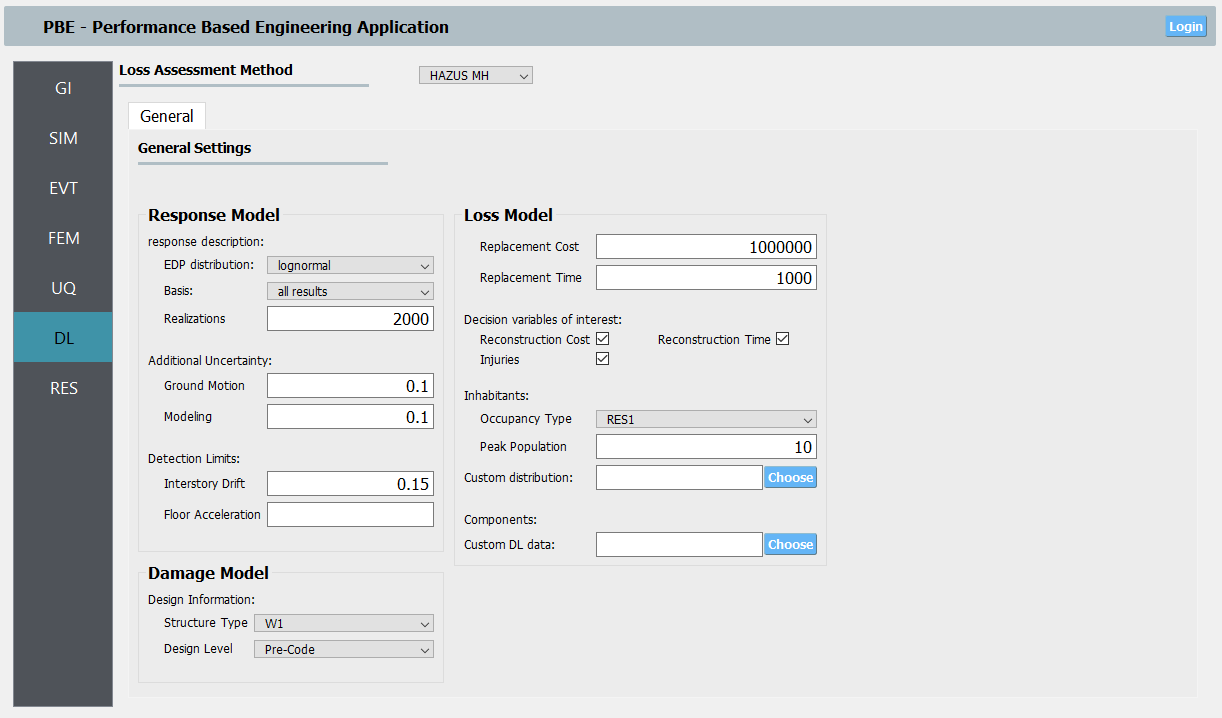
\includegraphics[width=0.95\textwidth]
    {installation/figures/test_input_dl.png} }
  \caption{Specifying the damage and loss model for the analysis.}
  \label{fig:input_dl}
\end{figure}
}{}

Now, click on the \texttt{RUN} button to start the calculation. 

\softwareSwitch{PBE}{
\begin{figure}[!htbp]
  \centering {
    \includegraphics[width=0.95\textwidth]
    {installation/figures/test_uq_res_pbe.png} }
  \caption{Results for test analysis. This tab will open automatically
  when the analysis completes, indicating a successful installation}
  \label{fig:show_results}
\end{figure}
}{}

\softwareSwitch{EE-UQ}{
\begin{figure}[!htbp]
  \centering {
    \includegraphics[width=0.7\textwidth]
    {installation/figures/test_uq_res.png} }
  \caption{Results for test analysis. This tab will open automatically
  when the analysis completes, indicating a successful installation}
  \label{fig:show_results}
\end{figure}
}{}

\softwareSwitch{WE-UQ}{
\begin{figure}[!htbp]
  \centering {
    \includegraphics[width=0.7\textwidth]
    {installation/figures/test_uq_res.png} }
  \caption{Results for test analysis. This tab will open automatically
  when the analysis completes, indicating a successful installation}
  \label{fig:show_results}
\end{figure}
}{}

If successful, the application will pause briefly while it runs the
analysis before automatically displaying the simulations results in
the \texttt{RES} tab, as shown
in \Cref{fig:show_results}. Remember, the results shown
in \Cref{fig:show_results} most likely will not be the same as
those from this local test since $V_{S_{30}}$ is a random variable and
the values realized in the simulations will be different while still
following the same distribution. In any case, if the simulations
completed and the \texttt{RES} tab shows simulation results, then
the \texttt{\getsoftwarename{}} App is properly installed and configured.

%===============================================================================


\chapter{Usage}
\label{chap:usage}
\input{usage/usage.tex}

\chapter{Theory and Implementation}
\label{chap:theory}
\input{theory_and_implementation/theory_and_implementation_PBE.tex}

\chapter{Source Code}
\label{chap:SourceCode}
\input{source_code/source_code.tex}

\chapter{User Training}
\label{chap:training}
\input{training/training.tex}

\chapter{Examples}
\label{chap:examples}
\input{examples/examples.tex}

\chapter{Verification and Validation}
\label{chap:vnv}
\input{ver_and_val/ver_and_val_PBE.tex}

\chapter{Requirements}
\label{chap:requirements}
This chapter outlines the general features of the \texttt{\getsoftwarename{}} application. We show when the features were introduced and what features and when you can expect to see in the future. This provides a roadmap of where this application has come from and where it is headed. The future features are highly dependent on user feedback. You are highly encouraged to contact us to discuss any new features you would like to see in the application.\\

\softwareSwitch{PBE}{
Note: All but the Damage and Loss (9) features overlap with the requirements for the EE-UQ application.\\
}{}

\Cref{tab:schedule} shows the scheduled release dates for this tool and includes the list of features provided in that release or what you can expect to see in future releases. The individual feature requirements are outlined in \Cref{tab:featureRequirements}. If you would like some additional features added, please contact us.
Additionally, we would appreciate any feedback on this tool. An anonymous
user survey is available \insertsurveylink{here}. \\

\softwareSwitch{PBE}{
    \begin{table}[hbt!]                    
      \centering
    \begin{adjustbox}{max width=0.7\textwidth}            
      \begin{tabular}{lll}                    
        \toprule          
          Version & 	Release	 & Requirements \\  \hline
          1.0	& October 2018   &	 1.1, 1.2, 2.1, 2.2, 2.3, 2.4, 2.5\\
                &                &   3.1, 4.1, 4.2, 5.1, 5.2, 6.1, 7\\
                &                &   9.1a, 9.2a-i, 9.3a-d, 9.4a-c\\ \hline
          1.1   & March 2019     &	 2.7a, 2.8a, 3.6, 6.3, 8.1\\
                &                &   9.1b, 9.3e-f\\ \hline
          1.2   & June 2019      &   2.7b, 9.3g, 10.1\\  \hline
          2.0   & September 2019 &   2.6, 2.7c, 2.7d, 2.8b, 3.2, 4.4\\
                &                &   6.2, 6.3, 8.2\\
                &                &   9.1c-e, 9.4d\\ \hline
      \end{tabular}
    \end{adjustbox}
      \caption{Schedule of Release}             
      \label{tab:schedule}                 
    \end{table}
}{
\softwareSwitch{EE-UQ}{
    \begin{table}[hbt!]                    
      \centering
    \begin{adjustbox}{max width=\textwidth}            
      \begin{tabular}{lll}                    
        \toprule          
          Version & 	Release	 & Requirements \\  \hline
          1.0	 & September 2018 &	1.1, 1.2, 2.1, 2.2, 2.3, 2.4, 2.5, 3.1, 4.1, 4.2, 5.1, 5.2, 6.1, 7\\  \hline
          1.1	 & March 2019     &	2.7a, 2.8a, 3.6, 6.3, 8.1\\  \hline
          1.2	 & June  2019      &	2.7b\\  \hline
          2.0	 & September 2019 &	2.6, 2.7c, 2.7d, 2.8b, 3.2, 4.4, 6.2, 6.3, 8.2\\  \hline
      \end{tabular}
    \end{adjustbox}
      \caption{Schedule of Release}             
      \label{tab:schedule}                 
    \end{table}
}{
    \begin{table}[hbt!]                    
      \centering
    \begin{adjustbox}{max width=\textwidth}            
      \begin{tabular}{lll}                    
        \toprule          
          Version & 	Release	 & Requirements \\  \hline
          1.0	 & July 2019 & 1.1, 1.2, 2.1, 2.2, 3.1, 3.6, 4.1, 4.2, 4.3, 4.1, 4.2, 4.3, 5.1, 7, 8.1, 9.1\\  \hline
      \end{tabular}
    \end{adjustbox}
      \caption{Schedule of Release}             
      \label{tab:schedule}                 
    \end{table}
}
}

\newpage
\softwareSwitch{WE-UQ}{
\begin{longtable}{| p{.05\textwidth} | p{.75\textwidth} | p{.08\textwidth} | p{.08\textwidth} |}
    \toprule
      \# & Description & Priority & Version \\ \hline
      1 & \textbf{Ability to simulate wind loads specific to each building and surrounding terrain} &  &  \\ 
	1.1 & Run on Local Machine (Mac and Windows) & M & 1.0 \\ \hline
	1.2 & Run on Stampede2 through DesignSafe utilizing Agave & M & 1.0 \\ \hline
	2 & \textbf{New tools for practice to determine wind loading effects validated against tests or other simulation methods} &  &  \\ \hline
	2.1 & Ability to select from multiple wind loading events and view UQ due to all the discrete events & M & 1.0  \\ \hline
	2.2 & Ability to select from synthetic wind loads &  &  \\
	 & a)     per Wittig \& Sinha (1975) & M & 1.0  \\ \hline
	3 & \textbf{Building Model Generation} &  & \\ \hline
	3.1 & Ability to use existing OpenSees model scripts. & M & 1.0 \\ \hline
	3.2 & Ability to define building and use Expert System to generate FE mesh of: &  &  \\
	 & a)     Concrete Shear Walls & M & UPDATE \\ 
	 & b)     Moment Frames & M & UPDATE \\ 
	 & c)     Braced Frames & M & UPDATE  \\ \hline
	3.3 & Ability to define building and use Machine Learning applications to generate FE mesh for: &  &  \\ 
	 & a)     Concrete Shear Walls & M & UPDATE \\ 
	 & b)     Moment Frames & M & UPDATE \\ 
	 & c)     Braced Frames & M & UPDATE  \\ \hline
	3.4 & Ability to specify connection details for member ends & M & UPDATE \\ \hline
	3.5 & Ability to define a user-defined moment-rotation response representing the connection details & D & UPDATE \\ \hline
	3.6 & Ability to quickly create a simple shear building model & D & 1.0 \\ \hline
	4 & \textbf{FEM} &  &  \\ \hline
	4.1 & Ability to specify OpenSees as FEM engine and to specify different analysis options. & M & 1.0 \\ \hline
	4.2 & Ability to provide own OpenSees Analysis script to OpenSees engine. & D & 1.0 \\ \hline
	4.3 & Ability to provide own Python script and use OpenSeesPy engine. & O & 1.0 \\ \hline
	4.4 & Ability to use alternative FEM engine. & M & UPDATE \\ \hline
	5 & \textbf{UQ - Method} &  &  \\ \hline
	5.1 & Ability to Use Dakota UQ engine with the Monte Carlo and LHS methods to perform sampling & M & 1.0 \\ \hline
	5.2 & Ability to Use alternative UQ engines & M & UPDATE \\ \hline
    6 & \textbf{UQ – Random Variables} &  &  \\ \hline
	6.1 & Ability to Define Variables of certain types: &  &  \\ 
	 & a)     Normal &  &  \\ 
	 & b)     Lognormal &  &  \\ 
	 & c)     Uniform & M  & 1.0 \\ 
	 & d)     Beta &  &  \\ 
	 & e)     Weibull &  &  \\ 
	 & f)     Gumbel &  &  \\ \hline
	6.2 & User defined Distribution & M & UPDATE \\ \hline
	6.3 & Define Correlation Matrix & M & UPDATE \\ \hline
	7 & Tool to allow user to load and save user inputs & M & 1.0 \\ \hline
    8 & \textbf{Engineering Demand Parameters} &  &  \\ \hline
	8.1 & Ability to Process own Output Parameters & M & 1.0 \\ \hline
	8.2 & Add to Standard Wind a variable indicating analysis failure & D & UPDATE  \\ \hline
    9 & \textbf{Ability to use a cyber based wind tool that supports performance based design} & & \\ \hline
    9.1 & Ability to generate floor loads using database-enabled design & M & 1.0 \\ \hline
    10 & \textbf{Misc.} &  &  \\ \hline
	10.1 & Simplify run local and run remote by removing workdir locations. Move to preferences & D & UPDATE  \\ \hline
	\bottomrule 
\caption{Feature Requirements (M=Mandatory, D=Desirable, O=Optional, P=Possible Future)}             
  \label{tab:featureRequirements}                 
\end{longtable}
}{
\begin{longtable}{| p{.07\textwidth} | p{.65\textwidth} | p{.08\textwidth} | p{.08\textwidth} |  p{.08\textwidth} |}
    \toprule
      \# & Description & Source & Priority & Version \\ \hline
      1 & \textbf{Ability to determine response of Building Subject to Earthquake hazard including formal treatment of randomness and uncertainty uncertainty} & GC & M  & 1.0  \\ \hline
      1.1 & Simulations able to utilize HPC resources & GC & M & 1.0 \\ \hline
      1.2 & Tool should incorporate data from www & GC & M & 1.0 \\ \hline
      1.3 & Tool available for download from web & GC & M & 1.0 \\ \hline
      2 & \textbf{Various Motion Selection Options} & SP & M & 1.0  \\ \hline
      2.1 & Ability to select from Multiple input motions and view UQ due to all the discrete events & GC & M & 1.0  \\ \hline
      2.2 & Ability to select from list of SimCenter motions & SP & M & 1.0 \\ \hline
      2.3 & Ability to select from list of PEER motions & SP & D & 1.0 \\ \hline
      2.4 & Ability to use OpenSHA and selection methods to generate motions & UF & D & 1.0 \\ \hline
      2.5 & Ability to Utilize Own Application in Workflow & SP & M & 1.0 \\ \hline
      2.6 & Ability to use Broadband & SP & D &  \\ \hline
      2.7  & Ability to include Soil Structure Interaction Effects & GC & M & 1.1 \\  \hline
      2.7.1  & 1D nonlinear site response with effective stress analysis & SP & M & 1.1  \\ \hline
      2.7.2  & Nonlinear site response with bidirectional loading & SP & M & 1.2 \\  \hline
      2.7.3  & Nonlinear site response with full stochastic characterization of soil layers & SP & M &  \\ \hline
      2.7.4 & Nonlinear site response, bidirectional different input motions  & SP & M &  \\  \hline
      2.7.5 & Building in nonlinear soil domain utilizing large scale rupture simulation & GC  & M &  \\  \hline
      2.7.5.1 & Interface using DRM method  & SP  & M &  \\  \hline
      2.8 & Utilize PEER NGA www ground motion selection tool  & UF & D & 2.0 \\ \hline
      2.9 & Ability to select from synthetic ground motions & SP & M & 1.0  \\
      2.9.1 & per Vlachos, Papakonstantinou, Deodatis (2017) & SP & D & 1.1  \\ 
      2.9.2 & per Dabaghi, Der Kiureghian (2017) & UF & D & 2.0 \\ \hline
	3 & \textbf{Building Model Generation} & GC & M & 1.0 \\ \hline
	3.1 & Ability to quickly create a simple nonlinear building model & GC & D & 1.1 \\ \hline
	3.2 & Ability to use existing OpenSees model scripts & SP & M & 1.0 \\ \hline
	3.3  & Ability to define building and use Expert System to generate FE mesh & SP & &  \\ \hline
	3.3.1 & Expert system for Concrete Shear Walls & SP & M &  \\ \hline
	3.3.2 & Expert system for Moment Frames & SP & M &  \\ \hline
	3.3.3 & Expert system for  Braced Frames & SP & M &   \\ \hline
	3.4 & Ability to define building and use Machine Learning applications to generate FE & GC &  &  \\ \hline
	3.4.1 & Machine Learning for Concrete Shear Walls & SP & M &  \\ \hline
	3.4.2 & Machine Learning for Moment Frames & SP & M &  \\ \hline
	3.4.3 & Machine Learning for Braced Frames & SP & M &   \\ \hline
	3.5 & Ability to specify connection details for member ends & UF & M &  \\ \hline
	3.6 & Ability to define a user-defined moment-rotation response representing the connection details & UF & D & 2.2 \\ \hline
	4 & \textbf{Perform Nonlinear Analysis} & GC & M & 1.0 \\ \hline
	4.1 & Ability to specify OpenSees as FEM engine and to specify different analysis options & SP & M & 1.0 \\ \hline
	4.2 & Ability to provide own OpenSees Analysis script to OpenSees engine. & SP & D & 1.0 \\ \hline
	4.3 & Ability to provide own Python script and use OpenSeesPy engine. & UF & O &  \\ \hline
	4.4 & Ability to use alternative FEM engine. & SP & M & 2.0 \\ \hline
	5 & \textbf{Uncertainty Quantification Methods} &  GC & M & 1.0  \\ \hline
	5.1 & \textbf{Various Forward Propogation Methods} & SP & M & 1.0  \\ \hline
	5.1.1 & Ability to use basic  Monte Carlo and LHS methods & SP & M & 1.0 \\ \hline
	5.1.2 & Ability to use Importance Sampling  & SP & M & 2.0 \\ \hline
	5.1.3 & Ability to use Gaussian Process Regression & SP & M & 2.0 \\ \hline
	5.1.4 & Ability to use Own External UQ Engine & SP & M &  \\ \hline
	5.2 & \textbf{Various Reliability Methods} & UF & M &  \\ \hline
	5.2.1 & Ability to use First Order Reliability method & UF & M &  \\ \hline
	5.2.2 & Ability to use Second Order Reliability method & UF & M & \\ \hline
	5.2.2 & Ability to use Surrogate Based Reliability & UF & M & \\ \hline
	5.2.3 & Ability to use Own External Application to generate Results & UF & M &  \\ \hline
	5.3 & \textbf{Various Sensitivity Methods} & UF & M &  \\ \hline
	5.3.1 & Ability to obtain Global Sensitivity Sobol's indices & UF & M &  \\ \hline
    6 & \textbf{Random Variables for Uncertainty Quantification} & GC & M & 1.0  \\ \hline
    6.1 & Ability to Define Variables of certain types: & SP & M & 1.0  \\ 
    6.1.1 & Normal & SP & M  & 1.0 \\ \hline
    6.1.2 & Lognormal & SP & M & 1.0 \\ \hline
    6.1.3 & Uniform & SP & M & 1.0  \\ \hline
    6.1.4 & Beta & SP & M & 1.0 \\ \hline
    6.1.5 & Weibull &  SP & M  & 1.0 \\ \hline
    6.1.6 & Gumbel &  SP & M & 1.0  \\ \hline
    6.2 & User defined Distribution & SP & M &  \\ \hline
    6.3 & Correlated Random Variables & SP & M &  \\ \hline
    6.4 & Random Fields & SP & M &  \\ \hline
     7 & Tool to allow user to load and save user inputs & SP & M & 1.0 \\ \hline
    8 & \textbf{Engineering Demand Parameters} &  &  \\ \hline
    8.1 & Ability to Process own Output Parameters & UF & M &   \\ \hline
    8.2 & Add to Standard Earthquake a variable indicating analysis failure & UF & D &   \\ \hline
    8.3 & Allow users to provide their own set of EDPs for the analysis. & UF & D & 2.0\\ \hline

9 & \textbf{Damage and Loss Assessment} & GC & M & 1.0\\ \hline
9.1 & Different Assessment Methods & GC & M & 2.0 \\ \hline
9.1.1 & Ability to perform component-based (FEMA P58) loss assessment for an earthquake hazard. & SP & M & 1.0 \\ \hline
9.1.2 & Ability to perform component-assembly-based (HAZUS MH) loss assessment for an earthquake hazard. & SP & D & 1.1 \\ \hline
9.1.3 & Ability to perform downtime estimation using the REDi methodology. & UF & D & \\ \hline
9.1.4 & Ability to describe building performance with additional decision variables from HAZUS (e.g., business interruption, debris) & SP & D &  \\ \hline
9.1.5 &  Ability to perform time-based assessment & GC & M &  \\ \hline
9.1.6 & Ability to perform damage and loss assessment for hurricane wind & GC & M &  \\ \hline
9.1.7 & Ability to perform damage and loss assessment for storm surge & GC & M &  \\ \hline
9.2 & Control & SP & M & 1.0 \\ \hline
9.2.1 & Allow users to set the number of realizations & SP & M & 1.0\\ \hline
9.2.2 &  Allow users to specify the added uncertainty to EDPs & SP & M & 1.0 \\ \hline
9.2.3 &  Allow users to decide which decision variables to calculate & SP & D & 1.0 \\ \hline
9.2.4 &  Allow users to set the number of inhabitants on each floor and customize their temporal distribution. & SP & D & 1.0 \\ \hline
9.2.5 &  Allow users to specify the boundary conditions of repairability. & SP & D & 1.0 \\ \hline
9.2.6 &  Allow users to control collapse through EDP limits. & SP & D & 1.0\\ \hline
9.2.7 &  Allow users to specify the replacement cost and time for the building. & SP & M & 1.0 \\ \hline
9.2.8 &  Allow users to specify EDP boundaries that correspond to reliable simulation results. & SP & D & 1.0\\ \hline
9.2.9 & Allow users to specify collapse modes and characterize the corresponding likelihood of injuries. & SP & D & 1.0\\ \hline
9.2.10 & Allow users to specify the collapse probability of the structure. & UF & M & 1.2\\ \hline
9.2.11 & Allow users to use empirical EDP data to estimate the collapse probability of the structure. & UF & M & 1.2\\ \hline
9.2.12 & Allow users to choose the type of distribution they want to estimate the EDPs with. & UF & D & 1.2\\ \hline
9.2.13 & Allow users to perform the EDP fitting only for non-collapsed cases. & UF & M & 1.2\\ \hline
9.2.14 & Allow users to couple response estimation with loss assessment. & UF & M & \\ \hline
9.3 & Component damage and loss information & SP & M & 1.0\\ \hline
9.3.1 & Make the component damage and loss data from FEMA P58 available. & SP & M & 1.0 \\ \hline
9.3.2 & Ability to use custom components for loss assessment. & SP & D & 1.0 \\ \hline
9.3.3 & Allow users to set different component quantities for each floor in each direction. & SP & D & 1.0 \\ \hline
9.3.4 & Allow users to set the number of identical component groups and their quantities within each performance group. & UF & D & 1.0 \\ \hline
9.3.5 & Use a generic JSON data format for building components that can be shared by component-based and component-assembly-based assessments. & SP & D & 1.1 \\ \hline
9.3.6 & Convert FEMA P58 and HAZUS component damage and loss data to the new JSON format and make it available with the tool. & SP & D & 1.1 \\ \hline
9.3.7 & Make component definition easier by providing a list of available components in the given framework (e.g. FEMA P58 or HAZUS) and not requesting inputs that are already available in the data files. & UF & D & 1.2 \\ \hline
9.3.8 & Make the component damage and loss data from FEMA P58 2nd edition available. & UF & M & 2.0 \\ \hline
9.3.9 & Improve component definition by providing complete control over every characteristic on every floor and in every direction & UF & D & 2.0 \\ \hline
9.3.10 & Allow users to view fragility and consequence functions in the application & UF & D &  \\ \hline
9.3.11 & Allow users to edit fragility and consequence functions in the application & UF & D &  \\ \hline
9.4 & Stochastic loss model & SP & M & 1.0 \\ \hline
9.4.1 & Allow the user to specify basic dependencies (i.e. independence or perfect correlation) between logically similar parts of the stochastic model (i.e. within component quantities or one type of decision variable, but not between quantities and fragilities) & SP & D & 1.0 \\ \hline
9.4.2 & Allow the user to specify basic dependencies between reconstruction cost and reconstruction time. & SP & D & 1.0 \\ \hline
9.4.3 & Allow the user to specify basic dependencies between different levels of injuries. & SP & D & 1.0 \\ \hline
9.4.4 & Allow the user to specify intermediate levels of correlation (i.e. not limited to 0 or 1) and provide a convenient interface that makes sure the specified correlation structure is valid. & SP & D & \\ \hline   
9.4.5 & Allow the user to specify the correlation for EDPs. & SP & D &  \\ \hline  

 M & \textbf{Misc.} & UF & M & 1.2  \\ \hline
   M.1 & Simplify run local and run remote by removing workdir locations. Move to preferences & UF & D & 1.2  \\ \hline
   M.2 & Add to EDP a variable indicating analysis failure & UF & D &   \\ \hline
   M.3 & Installer which installs application and all needed software & UF & M &   \\ \hline
 D & \textbf{Documentation} &  SP & M & 1.0 \\ \hline
 D.1 & Documentation exists on tool usage & SP & M & 1.1  \\ \hline
 D.2 & Video Exists demonstrating usage & SP & M & 1.1  \\ \hline
 D.3 & Verification Examples Exist & SP & M & 1.1  \\ \hline
  \bottomrule 
\caption{Requirements for PBE}
  \label{tab:featureRequirements}                 
\end{longtable}

Feature Requirements (M=Mandatory, D=Desirable, O=Optional, P=Possible Future)

\iffalse
\begin{longtable}{| p{.05\textwidth} | p{.75\textwidth} | p{.08\textwidth} | p{.08\textwidth} |}
    \toprule
      \# & Description & Priority & Version \\ \hline
      1 & \textbf{Ability to perform UQ on Building with Single Earthquake} &  &  \\ 
	1.1 & Run on Local Machine (Mac and Windows) & M & 1.0 \\ \hline
	1.2 & Run on Stampede2 through DesignSafe utilizing Agave & M & 1.0 \\ \hline
	2 & \textbf{Motion Selection} &  &  \\ \hline
	2.1 & Ability to select from Multiple Earthquakes and view UQ due to all the discrete events & M & 1.0  \\ \hline
	2.2 & Ability to select from list of SimCenter motions & M & 1.0 \\ \hline
	2.3 & Ability to select from list of PEER motions. & D & 1.0 \\ \hline
	2.4 & Ability to use OpenSHA and selection methods to generate motions & D & 1.0 \\ \hline
	2.5 & Ability to Utilize Own Application in Workflow & M & 1.0 \\ \hline
	2.6 & Ability to use Broadband & D & 3.0 \\ \hline
	\multirow{5}{*}{2.7} 
	& Ability to bring motion from rock to surface through soil &  &  \\ 
	 & a)     1d soil effective stress analysis though different soil layers & M & 1.1  \\ 
	 & b)     2d bidirectional loading & M & 1.2 \\ 
	 & c)     2d bidirectional with full stochastic characterization of soil layers & M & 2.0 \\
	 & d)     2d bidirectional with support for a set of input ground motions & O & 2.0 \\ 
	 \hline
	\multirow{5}{*}{2.8} 
	& Ability to select from synthetic ground motions &  &  \\
	 & a)     per Vlachos, Papakonstantinou, Deodatis (2017) & D & 1.1  \\ 
	 & b)     per Dabaghi, Der Kiureghian (2017) & D & 2.0 \\ \hline
	3 & \textbf{Building Model Generation} &  & 2.0 \\ \hline
	3.1 & Ability to use existing OpenSees model scripts. & M & 1.0 \\ \hline
	\multirow{5}{*}{3.2}  & Ability to define building and use Expert System to generate FE mesh of: &  &  \\
	 & a)     Concrete Shear Walls & M & 2.0 \\ 
	 & b)     Moment Frames & M & 2.0 \\ 
	 & c)     Braced Frames & M & 2.0  \\ \hline
	\multirow{5}{*}{3.3} & Ability to define building and use Machine Learning applications to generate FE mesh for: &  &  \\ 
	 & a)     Concrete Shear Walls & M & 2.0 \\ 
	 & b)     Moment Frames & M & 2.2 \\ 
	 & c)     Braced Frames & M & 2.3  \\ \hline
	3.4 & Ability to specify connection details for member ends & M & 2.2 \\ \hline
	3.5 & Ability to define a user-defined moment-rotation response representing the connection details & D & 2.2 \\ \hline
	3.6 & Ability to quickly create a simple shear building model & D & 1.1 \\ \hline
	4 & \textbf{FEM} &  &  \\ \hline
	4.1 & Ability to specify OpenSees as FEM engine and to specify different analysis options. & M & 1.0 \\ \hline
	4.2 & Ability to provide own OpenSees Analysis script to OpenSees engine. & D & 1.0 \\ \hline
	4.3 & Ability to provide own Python script and use OpenSeesPy engine. & O & 1.2 \\ \hline
	4.4 & Ability to use alternative FEM engine. & M & 2.0 \\ \hline
	5 & \textbf{UQ - Method} &  &  \\ \hline
	5.1 & Ability to Use Dakota UQ engine with the Monte Carlo and LHS methods to perform sampling & M & 1.0 \\ \hline
	5.2 & Ability to Use alternative UQ engines & M & 2.0 \\ \hline
    6 & \textbf{UQ – Random Variables} &  &  \\ \hline
	\multirow{5}{*}{6.1} & Ability to Define Variables of certain types: &  &  \\ 
	 & a)     Normal &  &  \\ 
	 & b)     Lognormal &  &  \\ 
	 & c)     Uniform & M  & 1.0 \\ 
	 & d)     Beta &  &  \\ 
	 & e)     Weibull &  &  \\ 
	 & f)     Gumbel &  &  \\ \hline
	6.2 & User defined Distribution & M & 2.0 \\ \hline
	6.3 & Define Correlation Matrix & M & 3.0 \\ \hline
	7 & Tool to allow user to load and save user inputs & M & 1.0 \\ \hline
	8 & \textbf{Engineering Demand Parameters} &  &  \\ \hline
	8.1 & Ability to Process own Output Parameters & M & 1.1  \\ \hline
	8.2 & Add to Standrard Earthquake a variable indicating analysis failure & D & 2.0  \\ \hline
\softwareSwitch{PBE}{9 & \textbf{Damage and Loss Assessment} & & \\ \hline
    \multirow{5}{*}{9.1} & Assessment Methods & & \\
     & a) Ability to perform component-based (FEMA P58) loss assessment for an earthquake hazard. & M & 1.0 \\
     & b) Ability to perform component-assembly-based (HAZUS MH) loss assessment for an earthquake hazard. & D & 1.1 \\
     & c) Ability to perform downtime estimation using the REDi methodology. & D & 2.0 \\
     & d) Ability to describe building performance with additional decision variables from HAZUS (e.g., business interruption, debris) & D & 2.0 \\
     & e) Ability to perform time-based assessment & M & 2.0 \\
     & f) Ability to perform loss assessment for other hazards & M & 2.0+ \\ \hline
    \multirow{5}{*}{9.2} & Control & & \\
     & a) Allow users to set the number of realizations & M & 1.0\\
     & b) Allow users to specify added of uncertainty to EDPs & M & 1.0 \\
     & c) Allow users to decide which decision variables to calculate & D & 1.0 \\
     & d) Allow users to set the number of inhabitants on each floor and customize their temporal distribution. & D & 1.0 \\
     & e) Allow users to specify the boundary conditions of repairability. & D & 1.0 \\
     & f) Allow users to control collapse through EDP limits. & D & 1.0\\
     & g) Allow users to specify the replacement cost and time for the building. & M & 1.0 \\
     & h) Allow users to specify EDP boundaries that correspond to reliable simulation results. & D & 1.0\\
     & i) Allow users to specify collapse modes and characterize the corresponding likelihood of injuries. & D & 1.0\\ \hline
	\multirow{5}{*}{9.3} & Component damage and loss information & & \\
	 & a) Make the component damage and loss data from FEMA P58 available. & M & 1.0 \\
	 & b) Ability to use custom components for loss assessment. & D & 1.0 \\
	 & c) Allow users to set different component quantities for each floor in each direction. & D & 1.0 \\
	 & d) Allow users to set the number of identical component groups and their quantities within each performance group. & D & 1.0 \\
     & e) Use a generic JSON data format for building components that can be shared by component-based and component-assembly-based assessments. & D & 1.1 \\
	 & f) Convert FEMA P58 and HAZUS component damage and loss data to the new JSON format and make it available with the tool. & D & 1.1 \\
	 & g) Make component definition easier by providing a list of available components in the given framework (e.g. FEMA P58 or HAZUS) and not requesting inputs that are already available in the data files. & D & 1.2 \\ \hline
	 \multirow{5}{*}{9.4} & Stochastic loss model & & \\
	 & a) Allow the user to specify basic dependencies (i.e. independence or perfect correlation) between logically similar parts of the stochastic model (i.e. within component quantities or one type of decision variable, but not between quantities and fragilities) & D & 1.0 \\
	 & b) Allow the user to specify basic dependencies between reconstruction cost and reconstruction time. & D & 1.0 \\
	 & c) Allow the user to specify basic dependencies between different levels of injuries. & D & 1.0 \\
	 & d) Allow the user to specify intermediate levels of correlation (i.e. not limited to 0 or 1) and provide a convenient interface that makes sure the specified correlation structure is valid. & D & 2.0 \\ \hline    
    10 & \textbf{Misc.} &  &  \\ \hline
	10.1 & Simplify run local and run remote by removing workdir locations. Move to preferences & D & 1.2  \\ \hline
}{  9 & \textbf{Misc.} &  &  \\ \hline
	9.1 & Simplify run local and run remote by removing workdir locations. Move to preferences & D & 1.2  \\ \hline
}
	\bottomrule 
\caption{Feature Requirements (M=Mandatory, D=Desirable, O=Optional, P=Possible Future)}             
  \label{tab:featureRequirements}                 
\end{longtable}
\fi
}


\chapter{Troubleshooting}
\label{chap:troubleshooting}
\input{troubleshooting/troubleshooting.tex}

%\nocite{*}

% \appendix
% \chapter{More Monticello Candidates}

\pagestyle{plain}
{
  \renewcommand{\thispagestyle}[1]{}	
  \printbibliography           
}

\end{document}
